% ==================================================
% Appendix: Uncertainty in cluster positions %
% ==================================================

%TODO : Organize figure positioning once you're done writing. 

\chapter[Cluster position uncertainty]{Uncertainty in cluster positions}
\label{appendix:clustering}

% Cluster def
% Cluster x from wires, cluster y from strips
% Cluster x uncertainty -- not needed in this
% Cluster y statistical uncertainty
% Cluster y systematic uncertainty depending on choice of fitting algorithm

% --------------------------------------------------
% \section{Cluster definition}
% --------------------------------------------------
%\label{sec:appendix_clustering_cluster_def}

%A cluster is a series of contiguous strip channels on a layer with non-zero amplitude, all part of the same trigger and having the same event number~\cite{lefebvre_thesis}. Clusters result from the drift of ionization products generate in the ionization avalanche caused by a muon~\cite{townsend_electricity_1915}. The peak-detector-output (PDO) of the signal on each strip of a cluster is fit with a Gaussian. The y-position of a particle as it passed through the layer is mean of the cluster, referred to here as the hit position.

% --------------------------------------------------
% \section{Effect of fit algorithm on cluster mean}
% --------------------------------------------------
% \label{sec:appendix_clustering_cluster_fit}

The clusters were fit with Guo's method~\cite{guo_simple_2011} and Minuit2 for ROOT~\cite{hatlo_developments_2005}. The difference in cluster means between the two algorithms is shown in figure~\ref{fig:mu_reclustering_minus_mu_cosmics}.

%TODO : Make this figure pretty with a nicer text box?
\begin{figure}
    \centering
    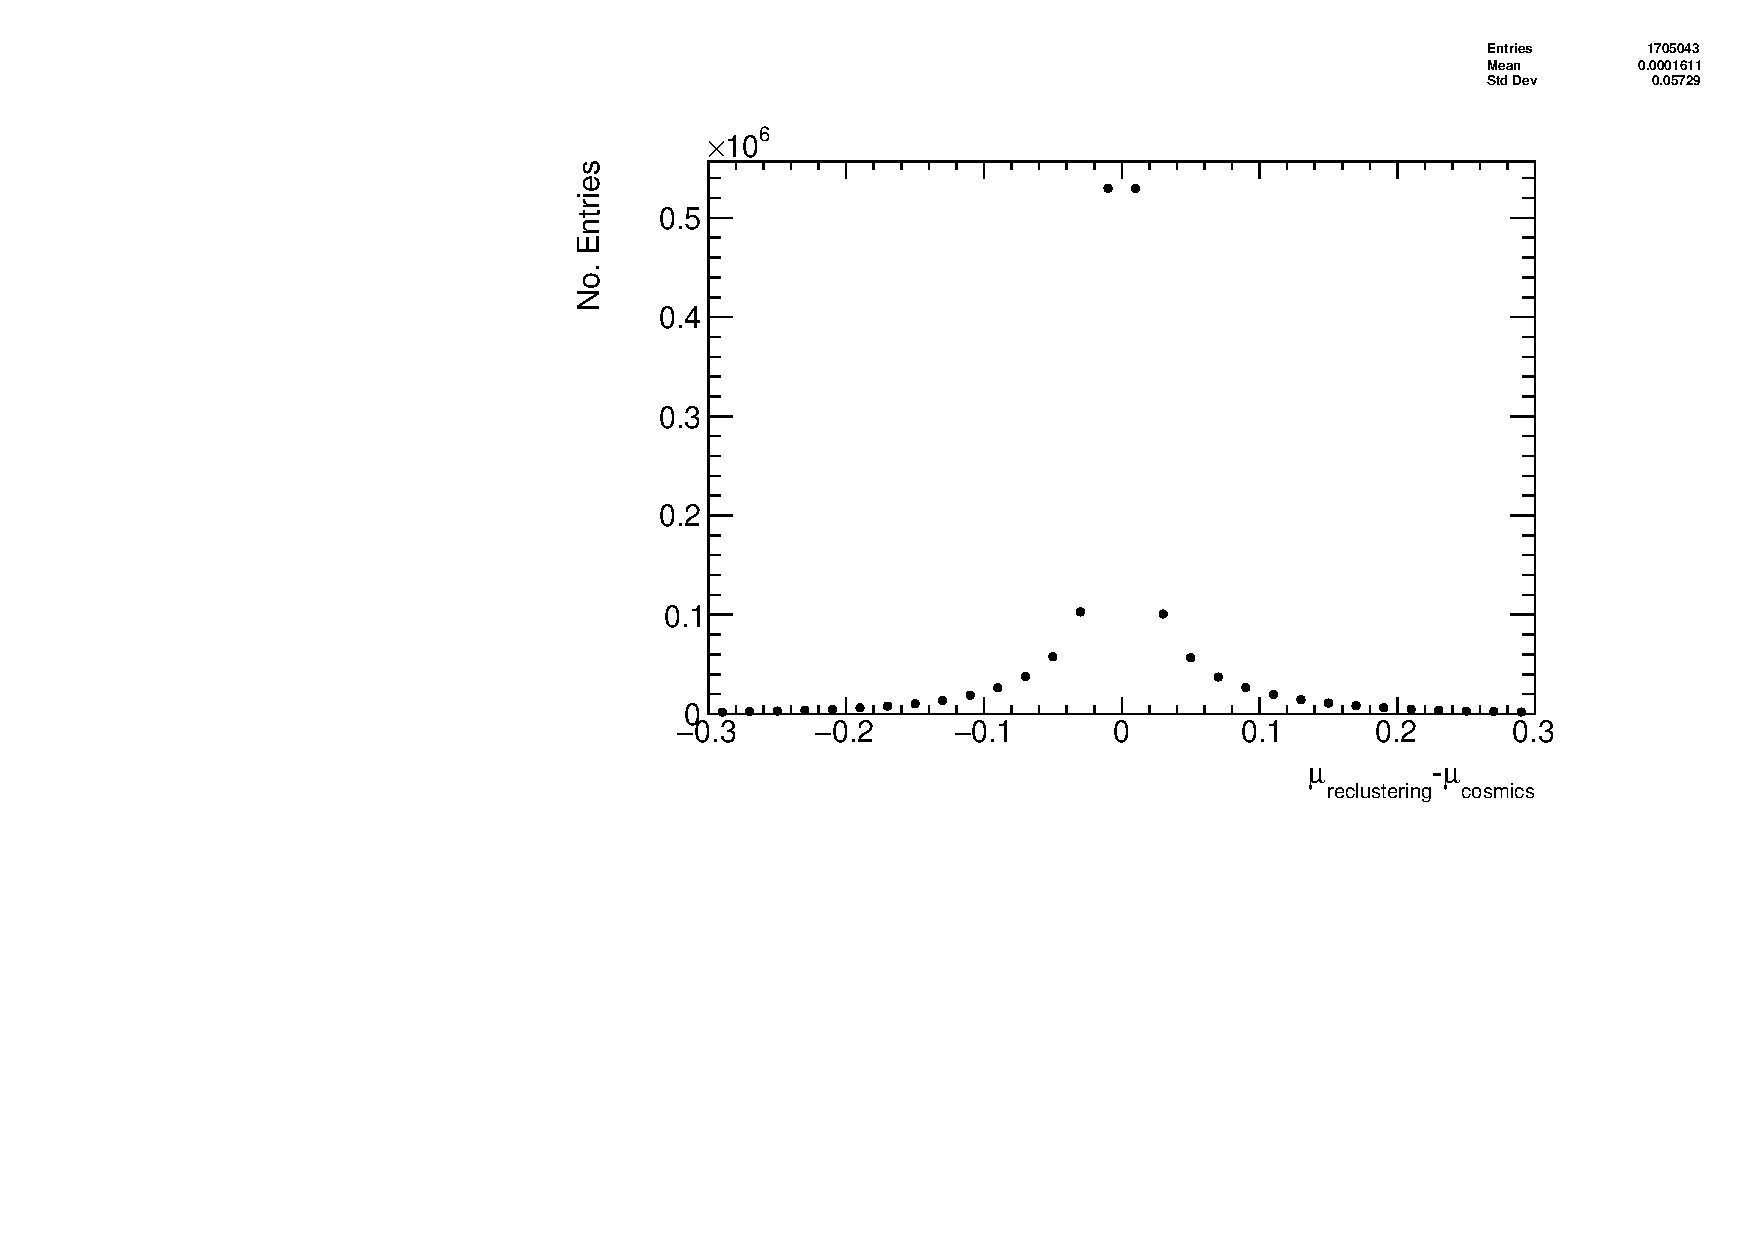
\includegraphics[width = \textwidth]{figures/figure_QL2P08_3100V_2021-05-21_reclustering_plots_mu_reclustering_minus_mu_cosmics.pdf}
    \caption{The difference between cluster means calculated with Guo's method~\cite{guo_simple_2011} in \package{tgc\_analysis/CosmicsAnalysis} and Minuit2 for ROOT~\cite{hatlo_developments_2005} in \package{strip\_position\_analysis/ReClustering} for data collected with QL2.P.8 at 3.1~kV.}
    \label{fig:mu_reclustering_minus_mu_cosmics}
\end{figure}

The RMS of the distribution in figure~\ref{fig:mu_reclustering_minus_mu_cosmics} is \SI{57}{\micro\meter}, which is much larger than the statistical uncertainty in the mean for the Minuit2 algorithm, which peaks around \SI{7}{\micro\meter}. An RMS of ~\SI{60}{\micro\meter} is common for data taken with most quadruplets at 3.1~kV. Therefore, the uncertainty in the reconstructed cluster $y$-coordinate is assigned \SI{60}{\micro\meter} due to variations in the reconstruction with different Gaussian fit algorithms.

% --------------------------------------------------
% \section{Effect of uncertainty in cluster mean on track residuals}
% --------------------------------------------------

%\label{sec:appendix_clustering_track_residuals}
%The uncertainty assigned to the hit position affected the uncertainty in the extrapolated/interpolated position of the track, and in the residuals. The bin size of the residual distributions was set to \SI{200}{\micro\meter} because that was the uncertainty in the residuals calculated from the tracks with the least favourable geometry (like tracks built from hits on layers 1 and 2 and extrapolated to layer 4). 